\section{La sustentation et l'aile}

\subsection{Les axes}
\subsubsection{Les 4 forces}
\begin{figure}[H]
		\centering
  		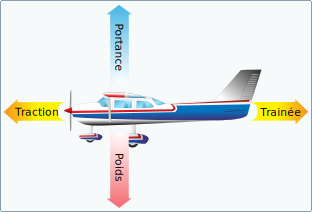
\includegraphics[width=0.8\textwidth]{04-Aerodynamique/img/forces.pdf}
  		\legende{Les 4 forces}{img:forces}	
\end{figure}

\subsection{L'aile}

\subsubsection{Description générale}
Toute aile est composée de plusieurs parties distinctes :
\begin{itemize}
	\item L'\gls{intrados} est la partie inférieure de l'aile. Lorsque l'aile se déplace dans une masse d'air, l'intrados est le siège d'une surpression.
	\item L'\gls{extrados} est la partie supérieure de l'aile. Lorsque l'aile se déplace dans une masse d'air, l'extrados est le siège d'une dépression (l'aile est aspirée vers le haut).
	\item Le \gls{bord d'attaque} \anglais{leading edge} est le point le plus en avant d'un profil d'aile. C'est à ce point que l'air entrera en contact en premier avec l'aile. Il s'agit généralement d'une surface  courbe.
	\item Le \gls{bord de fuite} \anglais{trailing edge} est le point le plus en arrière d'un profil d'aile.  Il s'agit généralement d'une pointe.
\end{itemize}

	\begin{figure}[H]
  	\centering
    \includegraphics[width=0.8\textwidth]{04-Aerodynamique/img/profilAile}
  	\legende{Profil d'une aile}{img:profilAile}
	\end{figure}	
	
	\astuce{Pour se souvenir où sont situés l'intrados et l'extrados : quand l'avion vole à plat, l'extrados fait face à l'extérieur de la planète, l'intrados regarde vers l'intérieur de la planète.} 
	
\subsubsection{Répartition des pressions autour d'une aile}
	\begin{figure}[H]
		\centering
  		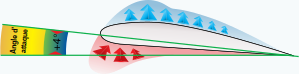
\includegraphics[width=0.8\textwidth]{04-Aerodynamique/img/pressionProfilSelonAngleAttaque4deg.pdf}
  		\legende{La pression autour d'une aile}{img:pressionProfilSelonAngleAttaque}
	\end{figure}	
	
	\subsubsection{Tourbillons marginaux}
	On a vu que l'extrados était le siège d'une dépression tandis que l'on retrouve une surpression sur l'intrados. Le saumon se trouve donc être l'interface entre une zone de surpression et une zone de dépression. Naturellement, l'air va chercher à rejoindre la zone de moindre pression, en contournant le saumon. Cela provoque un phénomène appelé tourbillon marginal ou vortex.
	\begin{center}
		\begin{minipage}[c]{1.0\linewidth}
		\begin{figure}[H]
		\begin{minipage}[c]{0.5\linewidth}
		\centering
		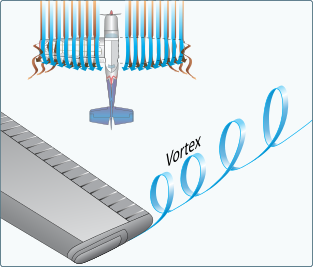
\includegraphics[width=0.95\linewidth]{04-Aerodynamique/img/vortexSchema.pdf}
		\legende{Schéma de la création d'un vortex}{img:vortexSchema}
		\end{minipage}
		\begin{minipage}[c]{0.5\linewidth}
		\centering
		\includegraphics[width=0.95\linewidth]{04-Aerodynamique/img/vortex.jpg}
		\legende{Mise en évidence d'un tourbillon marginal grâce à un fumigène}{img:vortex}
		\end{minipage}
		\end{figure}
		\end{minipage}
	\end{center}	
	
	Ce phénomène est indésirable car il produit une trainée, qui va donc diminuer la performance de l'aéronef (augmentation de la consommation et réduction de la vitesse pour un aéronef propulsé, augmentation du taux de descente en l'absence de moteur...). Pour limiter la production de ces tourbillons, on installe parfois des dispositifs appelés \textit{winglets} en bout d'aile. Ils constituent une sorte de barrière entre l'intrados et l'extrados.
	
	\begin{figure}[H]
  	\centering
    \includegraphics[width=0.6\textwidth]{04-Aerodynamique/img/Falcon7XWinglet}
  	\legende{Winglets en bout d'ailes d'un Falcon 7X}{img:Falcon7XWinglet}
	\end{figure}	
	
	\info{L'intensité des tourbillons marginaux produit par un aérodyne est directement proportionnelle à son poids.}
	
	\alert{Les tourbillons marginaux constituent une menace : un aéronef léger qui traverserait les tourbillons d'un aéronef plus lourd pour être retourné ou se casser en raison de la violence de ces phénomènes. Pour cette raison, le contrôle aérien assure une séparation entre 2 aéronefs qui se suivent lorsque le suivant est d'une catégorie de masse inférieure.}
	
	\subsubsection{Allongement d'une aile}
	On a vu que les tourbillons marginaux se formaient en bout d'aile. Si on imagine une aile (fictive) infinie, il n'y aurait pas de saumon pour faire l'interface entre l'intrados et l'extrados, et donc pas de formation de tourbillon marginal !
	
	Pour réduire les tourbillons marginaux, on peut donc augmenter l'allongement d'une aile, c'est à dire le rapport qu'il existe entre la corde de profil moyenne et la longueur de l'aile. Plus une aile est allongée, moins elle génère de tourbillons marginaux et donc de trainée liée à ce phénomène. Cela explique pourquoi les planeurs performants, mais aussi les avions de ligne (pour lesquels on veut minimiser les sources de trainée) ont des ailes très longues.
	
	L'allongement d'une aile $\lambda$ (sans unité) se calcule avec la formule suivante :
	
	 \begin{center}
		\huge{$\lambda = \dfrac{b^2}{S}$}
	\end{center}
	
	avec :
	\begin{itemize}
		\item $b$ : l'envergure de l'aile en $m$
		\item $S$ : la surface portante en $m^2$
	\end{itemize}
	

	
	\exemple{Le planeur EB29 existe avec 3 envergures différentes, et permet d'illustrer l'impact de l'allongement sur la traînée, en étudiant la valeur de la finesse (voir paragraphe \ref{chap:aero:finesse} \nameref{chap:aero:finesse}).
    \begin{table}[H]
	\centering
	\begin{tabular}{|c|c|c|c|}
		\hline
		\textbf{Envergure} & \textbf{Surface alaire} & \textbf{Allongement} & \textbf{Finesse max} \\ 
		\hline
		\hline
		$25,3~m$ & $15,4~m^2$ & $41,6$ & $63$ \\
		\hline
		$28,3~m$ & $16,5~m^2$ & $48,5$ & $66$ \\
		\hline
		$29,3~m$ & $16,8~m^2$ & $51,1$ & $68$ \\
		\hline
	\end{tabular}
	\legende{Impact de l'allongement sur la trainée, et donc la finesse, pour les 3 versions du planeur EB29}{tbl:FinesseEb29}
	\end{table}}
	

\subsection{La portance}
Sur un aérodyne, on cherche à générer avec l'aile une force orientée vers le haut, donc opposée au poids. Cette force est nommée portance.

On s'intéresse dans le graphique ci dessous à la valeur de la portance en fonction de l'incidence de l'aile. Cela permet d'extraire un coefficient nommé $C_z$.

\info{Les valeurs de $C_z$ sont obtenues de façon expérimentale en soufflerie.}

   \begin{figure}[H]
		\centering
  		\includegraphics[width=0.65\textwidth]{04-Aerodynamique/img/portanceTraineeFinesse_portance.pdf}
  		\legende{Portance en fonction de l'angle d'incidence de l'aile}{img:portanceTraineeFinesse}
	\end{figure}	
	
	On constate sur ce graphique que la valeur du coefficient de portance augmente avec l'incidence pour atteindre une valeur maximale après laquelle il chute rapidement. Cette chute rapide est liée au décollement des filets d'air, et donc à la force de portance qui s'applique sur une surface réduite de l'extrados. Une fois la totalité des filets décollés, la portance devient nulle : on a atteint l'incidence de décrochage.	
	
	\info{Sur la plupart des profils d'aile, le coefficient de portance maximum est obtenu entre 20 et 25° d'incidence.}
	
	\subsubsection{Décrochage}
	Le décrochage correspond à la baisse brutale de la portance générée par l'aile. Au moment du décrochage, la portance devient pratiquement nulle.
	%TODO
	
	\begin{figure}[H]
		\centering
  		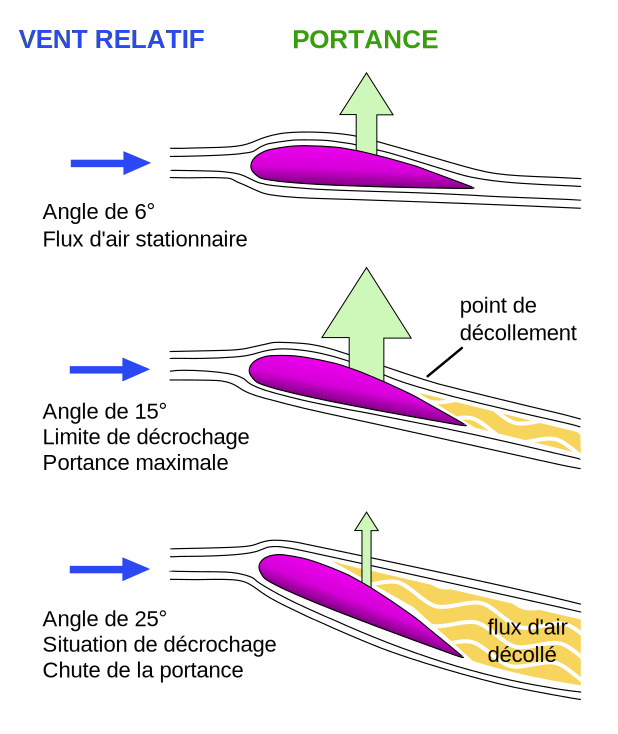
\includegraphics[width=0.6\textwidth]{04-Aerodynamique/img/portanceDecrochage.pdf}
  		\legende{Filets d'air sur une aile jusqu'au décrochage}{img:portanceDecrochage}
	\end{figure}	
	
	\alert{Le décrochage est causé par l'atteinte de l'incidence maximale du profil. Au dessus de l'incidence de décrochage, une aile ne porte plus quelque soit la vitesse.}

\subsubsection{Expression algébrique de la portance}
	\begin{center}
		\huge{$Z = \dfrac{1}{2}\rho S V^2 C_z$}
	\end{center}
	
	avec : \begin{itemize}
	\item $Z$ : valeur de la portance en $N$ (newtons)
	\item $\rho$ : densité de l'air en $kg/m^3$ ($\sim 1,2~kg/m^3$),
	\item $S$ : surface de l'aile en $m^2$,
	\item $V$ : vitesse en $m/s$,
	\item $C_z$ : coefficient de portance (sans unité), valeur liée à la forme de l'aile et à l'incidence.
	\end{itemize}
	

\subsection{La traînée}\label{chap:aero:trainee}
En physique, les phénomènes désirés s'accompagnent généralement de phénomènes indésirables. La trainée n'échappe pas à cette règle, et elle s'accompagne toujours d'un phénomène qui s'oppose à l'avancée de l'aile dans la masse d'air : la trainée induite (sous entendu induite par la portance).

Comme pour la portance, on s'intéresse à la valeur d'un coefficient qui caractérise la trainée, le $C_x$, en fonction de l'incidence de l'aile.
\begin{figure}[H]
		\centering
  		\includegraphics[width=0.65\textwidth]{04-Aerodynamique/img/portanceTraineeFinesse_trainee.pdf}
  		\legende{Trainée en fonction de l'angle d'incidence de l'aile}{img:portanceTraineeFinesse}
	\end{figure}	
	
	On constate sur le graphique ci dessus que la trainée augmente de façon continue avec l'augmentation de l'incidence de l'aile.

\subsubsection{Expression algébrique de la traînée}
	Il est possible d'exprimer la valeur de la trainée par une formule suivante :

	\begin{center}
		\huge{$X = \dfrac{1}{2}\rho S V^2 C_x$}
	\end{center}
	
	\begin{itemize}
	\item $X$ : trainée en $N$ (newtons)
	\item $\rho$ : densité de l'air en $kg/m^3$ ($\sim 1,2~kg/m^3$),
	\item $S$ : surface de l'aile en $m^2$,
	\item $V$ : vitesse en $m/s$,
	\item $C_x$ : coefficient de traînée (sans unité), valeur liée à la forme de l'aile et à l'incidence.
	\end{itemize}
	
	On constate que l'expression de la portance et de la traînée sont identiques au facteur $Cx$ et $Cz$ près. La portance et la traînée évoluent donc pendant le vol de la même façon.
	
	\subsubsection{Trainée totale}\label{chap:aero:traineeTotale}
	La trainée induite par l'aile n'est pas la seule composante de trainée qui freine l'aérodyne. Il faut ajouter à cette trainée des trainées dites \textit{parasites} issues des frottements de l'air sur les composants de la cellule : fuselage, nacelles moteur...
	
	\begin{figure}[H]
		\centering
	\begin{tikzpicture}[font=\sffamily]
 		\path[3d pie chart/.cd,radius=4cm,h=1.5cm,alpha0=45,
 		colors={"green","yellow","blue","violet","teal","pink"}] 
 		pic{3d pie chart={5/Composants de l'aile,18/Fuselage,18/Traînée de frottement de la forme,4/Nacelles moteur,11/Empennage,44/Traînée induite}};
	\end{tikzpicture}
	\legende{Répartition des composantes de la trainée totale (avion de ligne, vitesse de croisière)}{img:traineeTotale}
	\end{figure}	
	
	Compte tenu de l'importance relative des traînées parasites par rapport à la traînée induite, les bureaux d'études s'attachent à minimiser au maximum les trainées parasites en travaillant l'aérodynamisme de l'ensemble des composants de la cellule.
	
\subsection{La finesse}\label{chap:aero:finesse}
La finesse exprime le rapport entre la portance et la traînée. Il est possible de calculer la finesse pour n'importe quelle incidence d'une aile en calculant le rapport $\dfrac{C_z}{C_x}$.

Il s'agit en quelque sorte d'un coefficient qui indique l'efficacité d'une aile, et par extension, d'un aérodyne.

En pratique, la finesse peut également se calculer de façon expérimentale en vol, pour un aérodyne complet. Moteur coupé, la finesse  correspond au rapport de la distance parcourue sur l'altitude perdue. Par exemple, un appareil qui parcours $4,5~km$ en perdant $500~m$ d'altitude aura une finesse de $\dfrac{4,5}{0,5} = 9$. Cette finesse "totale" prend en compte la trainée induite par l'aile mais également toutes les autres trainées qui s'appliquent sur l'aéronef : trainée de frottement, trainé de forme ou encore trainée d'onde (lors de l'approche du vol supersonique).

\exemple{\begin{table}[H]
	\centering
	\begin{tabular}{|l|c|}
		\hline
		 \centering\textbf{Appareil} & \textbf{Finesse} \\
		\hline
		\hline
		Avion léger (DR400) & 9 \\
		\hline
		Avion de chasse (Rafale) & 5 \\
		\hline
		Hélicoptère & 2 \\
		\hline
		Avion de ligne (A330) & 30 \\
		\hline
		Parapente & 8 à 10 \\
		\hline
		Deltaplane & 15 \\
		\hline
		Planeur école & 40 à 50 \\
		\hline
		Planeur de compétition (EB29) & 60 à 70 \\
		\hline
  Concorde & \begin{tabular}{@{}c@{}}4 à 6 au décollage/en montée\\ 12 en subsonique \\ 7.5 en supersonique\end{tabular} \\
  \hline
		Navette spatiale & \begin{tabular}{@{}c@{}}1 en hypersonique \\ 2 en supersonique \\ 4.5 en subsonique\end{tabular} \\
		\hline
	\end{tabular}
	\caption{Quelques valeurs de finesse typiques}
	\end{table}}
	

\subsection{Polaire d'une aile}
Il est possible de tracer sur un graphique la portance ($C_z$) en fonction de la traînée ($C_x$) (voir également \href{\urlSite /polaireCxCz.html}{cette activité en ligne}\footnote{\urlSite /polaireCxCz.html} qui illustre la construction de la polaire).

\begin{figure}[H]
		\centering
  		\includegraphics[width=0.5\textwidth]{04-Aerodynamique/img/polaireAileMeilleureFinesse.pdf}
  		\legende{Polaire d'une aile, avec point de meilleure finesse}{img:polaireAileMeilleureFinesse}
\end{figure}	

Obtenue en traçant la portance $C_z$ en fonction de la traînée $C_x$. On peut identifier sur cette courbe plusieurs points caractéristiques :
 		\begin{itemize}
 			\item $A$ : $Cz = 0 \Rightarrow$ portance nulle
 			\item $B$ : traînée $C_x$ minimale
 			\item $C$ : $\dfrac{C_z}{C_x}$ minimum $\Rightarrow$ finesse maximale
 			\item $D$ : portance $C_z$ maximale
 			\item $E$ : décrochage
 		\end{itemize}
 		
 		\subsubsection{Polaire avion complet}
 		Comme indiqué dans \ref{chap:aero:traineeTotale} \nameref{chap:aero:traineeTotale}, des traînées parasites s'ajoutent aux traînées induites par l'aile. On peut tracer la polaire qui prend en compte ces 2 types de trainées. Il en résulte une polaire translatée vers la droite. La valeur de la translation est d'autant plus importante que les trainées parasites le sont par rapport à la trainée induite.
 		
 		\begin{figure}[H]
		\centering
  		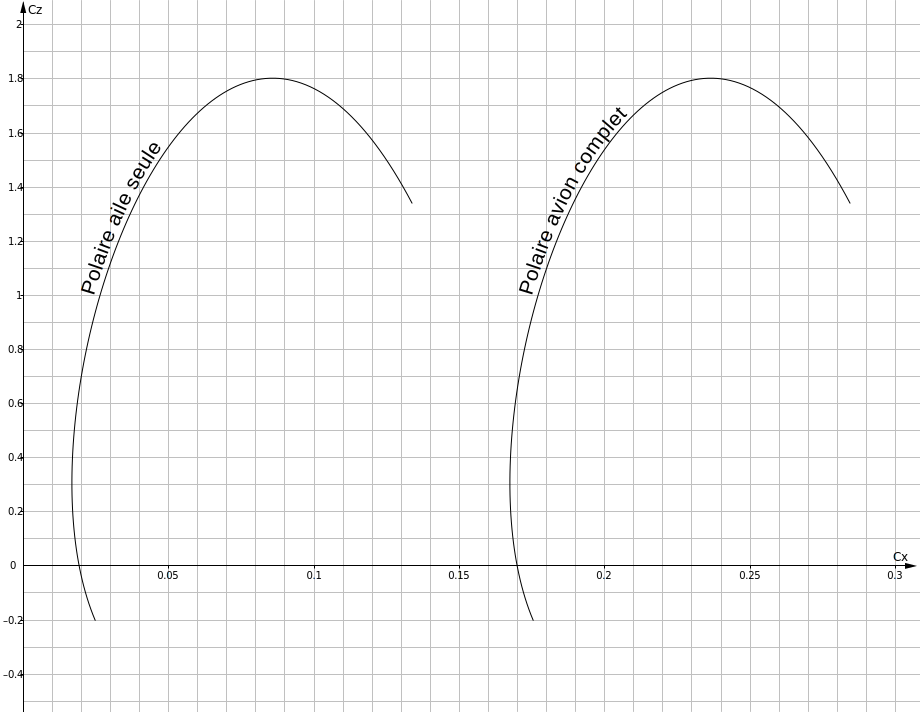
\includegraphics[width=0.95\textwidth]{04-Aerodynamique/img/polaireAvion.pdf}
  		\legende{Conséquence de la prise en compte de la trainée totale sur la polaire}{img:polaireAvion}
		\end{figure}

\subsection{Dispositifs hypersustentateurs et destructeurs de portance}\label{chap:aero:hyperHypoSutentateurs}
	\subsubsection{Dispositifs hypersustentateurs}
	Lors des phases d'atterrissage et de décollage, il est souhaitable de pouvoir évoluer à la vitesse la plus faible possible.	On peut obtenir cela grâce à une plus grande surface d'aile, ou concevoir l'aile pour augmenter son $C_z$. Mais, comme on l'a vu, toute augmentation du coefficient de portance ou de la surface de l'aile se fait au prix d'une augmentation de la traînée, indésirable en croisière (réduction des performances de montée, de vitesse maximale, augmentation de la consommation...).
	
	La solution consiste à modifier ces 2 paramètres (surface, $C_z$) uniquement quand on souhaite pouvoir voler moins vite. Cela est obtenu grâce aux dispositifs hypersustentateurs, qui sont de 2 types : \begin{itemize}
	\item volets \anglais{flaps}, situés sur ou à proximité du bord de fuite,
	\item becs \anglais{slats}, situés sur le bord d'attaque.
	\end{itemize}
	
	Ces dispositifs sont actionnés (par l'équipage, ou dans certains cas, automatiquement) pour le décollage, sont rentrés durant la montée, puis sont ressortis en vue de l'atterrissage. Sur la plupart des appareils, il est possible de sélectionner plusieurs "niveaux" de sortie de ces dispositifs. Ils sont généralement sortis de façon plus importante pour l'atterrissage, phase où l'augmentation de la traînée est moins problématique (au décollage, la traînée grève les performances de montée).
	
	La commande est transmise à ces surfaces par un jeu de tringles, ou sont motorisés par des systèmes électriques ou hydrauliques. \\
	
	\definition{Lorsqu'un appareil a tous ses dispositifs hypersustentateurs rentrés, on dit qu'il est en  \textbf{\gls{configuration lisse}}.}
	
		\paragraph{\Gls{volet}s}
			\subparagraph{Volets de courbure}
			Le type le plus simple sont les volets de courbure. Ces volets modifient le profil de l'aile en augmentant la courbure de l'aile à proximité du bord de fuite. Ces volets augmentent sensiblement le coefficient de portance, mais aussi la traînée.
		\begin{figure}[H]
			\centering
  			\includegraphics[width=0.4\textwidth]{04-Aerodynamique/img/hypersustentateurs/voletsDeCourbure.pdf}
  			\legende{Volets de courbure}{img:voletsDeCourbure}	
		\end{figure}
		
			\subparagraph{Volets d'intrados}
		Les volets d'intrados sont moins fréquemment utilisés sur les avions modernes. Ils augmentent la portance mais également la traînée dans des proportions très importantes. Ce type de volet est souvent assimilé à des aérofreins. 
		\begin{figure}[H]
			\centering
  			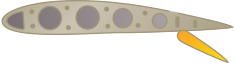
\includegraphics[width=0.4\textwidth]{04-Aerodynamique/img/hypersustentateurs/voletDIntrados.pdf}
  			\legende{Volets d'intrados}{img:voletDIntrados}	
		\end{figure}
		
			\subparagraph{Volets à fente}
			Le volet à fente se déploie sur le bord de fuite. Il augmente donc la portance en modifiant la surface de l'aile.
		\begin{figure}[H]
			\centering
  			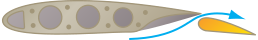
\includegraphics[width=0.4\textwidth]{04-Aerodynamique/img/hypersustentateurs/voletFowler.pdf}
  			\legende{Volets à fente}{img:voletFowler}	
		\end{figure}
		
			\subparagraph{Volets Fowler}
			Le volet Fowler (du nom de son inventeur américain Harlan Fowler) combine le volet à fente et le volet de cambrure. Il se déploie sur le bord de fuite puis s'abaisse vers le bas. Il augmente donc la portance en modifiant la surface de l'aile puis la cambrure (donc le $C_z$).
		
		\begin{figure}[H]
			\centering
  			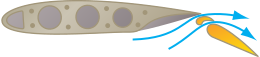
\includegraphics[width=0.4\textwidth]{04-Aerodynamique/img/hypersustentateurs/voletFowlerAFente.pdf}
  			\legende{Volets Fowler}{img:voletFowlerAFente}	
		\end{figure}
		
		\paragraph{\Gls{bec}s}
		Les becs de bord d'attaque sont des surfaces qui sortent à l'avant de l'aile. Ils augmentent la surface de l'aile.
		\begin{figure}[H]
			\centering
  			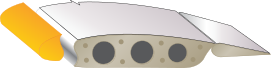
\includegraphics[width=0.4\textwidth]{04-Aerodynamique/img/hypersustentateurs/becs.pdf}
  			\legende{Becs de bord d'attaque}{img:becs}	
		\end{figure}
		
	\subsubsection{Les aérofreins}
	Les aérofreins \anglais{air brakes} sont des dispositifs situés sur les ailes ou sur le fuselage et dont l'objectif est d'augmenter la traînée. Ils permettent d'augmenter le taux de descente sans augmenter la vitesse.
	
	Les aérofreins sont généralement installés sur les avions de ligne, les planeurs ou encore les navettes spatiales.
	
	\begin{figure}[H]
	\begin{minipage}[c]{0.5\linewidth}
	\includegraphics[width=\linewidth]{04-Aerodynamique/img/afPlaneur.jpg}
	\legende{Planeur avec aérofreins de voilure déployés}{img:afPlaneur}
	\end{minipage}
	\hfill
	\begin{minipage}[c]{0.5\linewidth}
	\includegraphics[width=\linewidth]{04-Aerodynamique/img/afBae146.jpg}
	\legende{Aérofreins de cône de queue déployés}{img:afBae146}
	\end{minipage}
	\end{figure}
		
	\subsubsection{Dispositifs destructeurs de portance}
	Les dispositifs destructeurs de portance \anglais{spoilers} annulent totalement la portance et augmentent de façon importante la traînée.
	
	Ils sont généralement utilisés à l'atterrissage sur les avions de ligne pour plaquer l'aéronef au sol, et donc augmenter le poids supporté par le train d'atterrissage, ce qui augmente l'adhérence et donc l'efficacité du freinage.
	
	\begin{figure}[H]
	\centering
	\includegraphics[width=0.5\linewidth]{04-Aerodynamique/img/spoilerA320.jpg}
	\legende{A320 avec spoilers déployés}{img:spoilerA320}
	\end{figure}
	
\subsection{Stabilité}
	Sur un aéronef, il existe 2 points d'application des forces dont l'importance est capitale :
	\begin{itemize}
		\item le centre de gravité : c'est la que s'applique le poids,
		\item le foyer ou centre de portance : c'est le point ou s'applique le portance qui s'oppose au poids.
	\end{itemize}
	
	Le foyer a une position fixe : le vecteur qui représente la portance s'applique toujours en un même point.
	
	Le centre de gravité lui, a une position variable. En fonction de la masse de l'aéronef, le centre de gravité avance ou recule sur l'axe longitudinal de l'appareil. \\
	
	C'est la différence de position entre ces 2 centres qui rend l'avion pilotable, grâce aux forces aérodynamiques de déportance qui s'exercent sur la gouverne de profondeur. \\
	
	Il faut donc voir un aéronef comme une balance dont le pivot serait le foyer et dont chaque plateau serait représenté par le centre de gravité d'une part, et le point d'application de la déportance de la gouverne de profondeur d'autre part.
	
	\begin{figure}[H]
		\centering
  		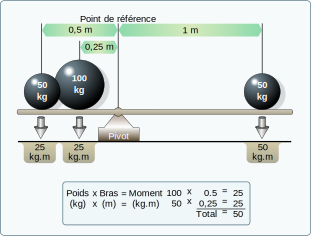
\includegraphics[width=0.5\textwidth]{04-Aerodynamique/img/balanceCentrage.pdf}
  		\legende{Balance et bras de levier}{img:balanceCentrage}	
	\end{figure}
	
	En agissant sur la valeur de la déportance, le pilote peut donc faire varier l'assiette de l'avion.
	
	\begin{figure}[H]
		\centering
  		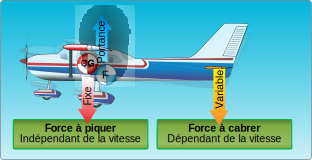
\includegraphics[width=0.8\textwidth]{04-Aerodynamique/img/centrage.pdf}
  		\legende{Centrage}{img:centrage}	
	\end{figure}
	
	On perçoit bien que la position du centre de gravité, qui est modifiable en changeant la position des masses dans l'aéronef, est un paramètre vital pour la capacité à contrôler l'assiette de l'aéronef : si le centre de gravité est trop en avant, la capacité de déportance de la gouverne de profondeur sera dépassée, et l'avion piquera du nez. A l'inverse, si le centre de gravité est trop en arrière (mais toujours en avant du foyer), une faible variation de l'effort de déportance de la gouverne de profondeur aura un effet important sur l'assiette (faible bras de levier entre le centre de gravité et de foyer). \\
	
	On comprend aussi que le vol est impossible si le centre de gravité se retrouve, de façon extrême, à l'arrière du foyer. Dans un tel cas, l'un des plateau de la balance sera toujours vide, toutes les forces orientées vers le bas se concentrant du même côté du pivot.
	
	\href{\urlSite /centrage.html}{Cette activité en ligne}\footnote{\urlSite /centrage.html} permet d'expérimenter l'impact du centrage et du calage de la gouverne de profondeur sur l'attitude de l'aéronef.
	\begin{figure}[H]
		\centering
  		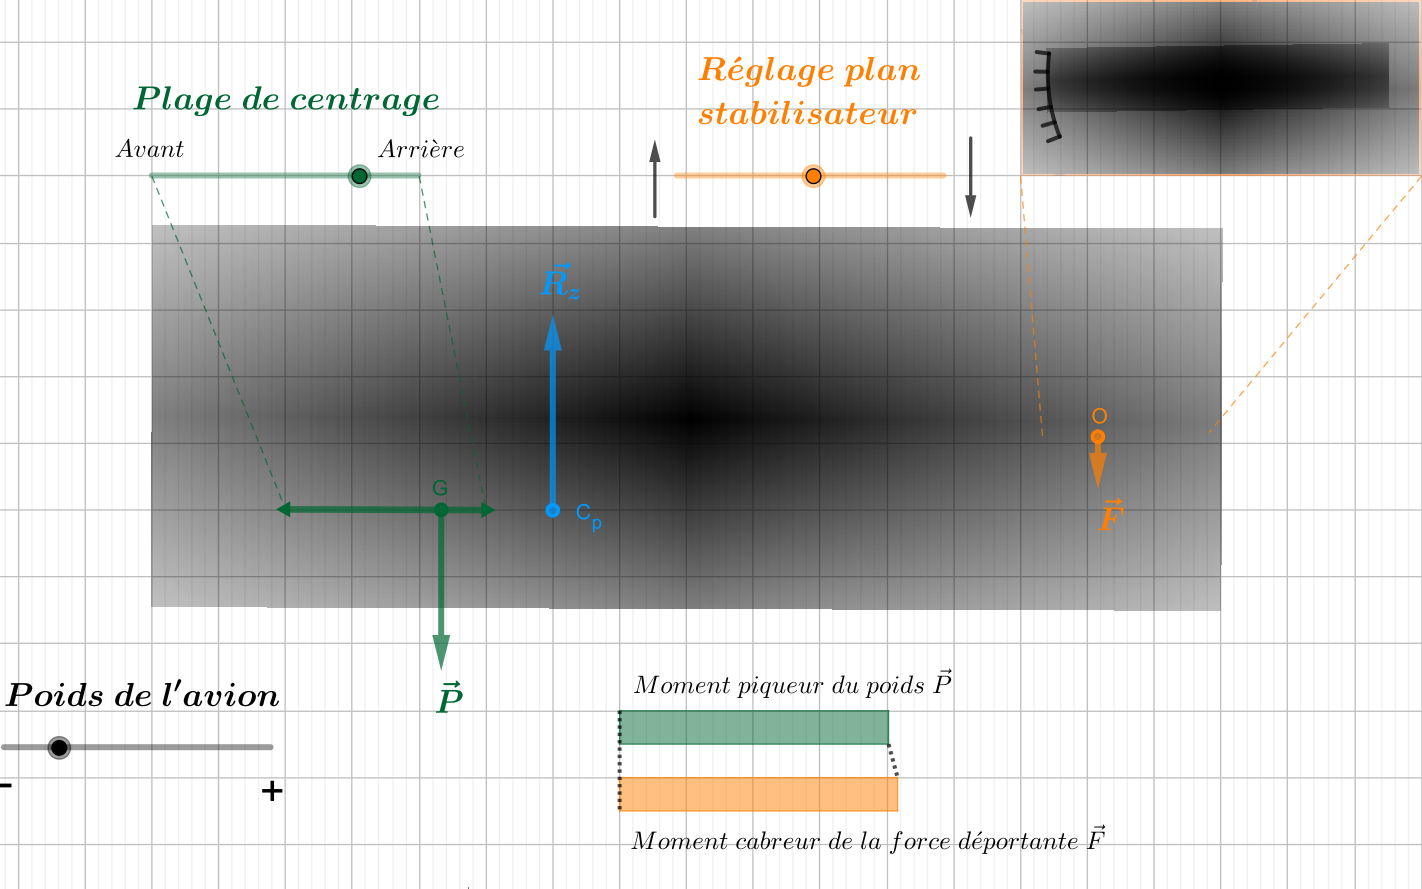
\includegraphics[width=0.8\textwidth]{04-Aerodynamique/img/centrageGgb.pdf}
  		\legende{Activité Geogabra : centrage}{img:centrageGgb}	
	\end{figure}
	
	\alert{Un centre de gravité en avant augmente la stabilité mais réduit la maniabilité. \\Un centre de gravité en arrière réduit la stabilité mais augmente la maniabilité. Par ailleurs, un centrage arrière réduit également la consommation. En effet, en centrage arrière, la profondeur à besoin de générer moins de déportance, elle génère donc également moins de trainée.}
	
	
	